\subsection{M.PC.6 - Variazione del budget tra preventivo e consuntivo}
\begin{figure}[H]
    \centering
    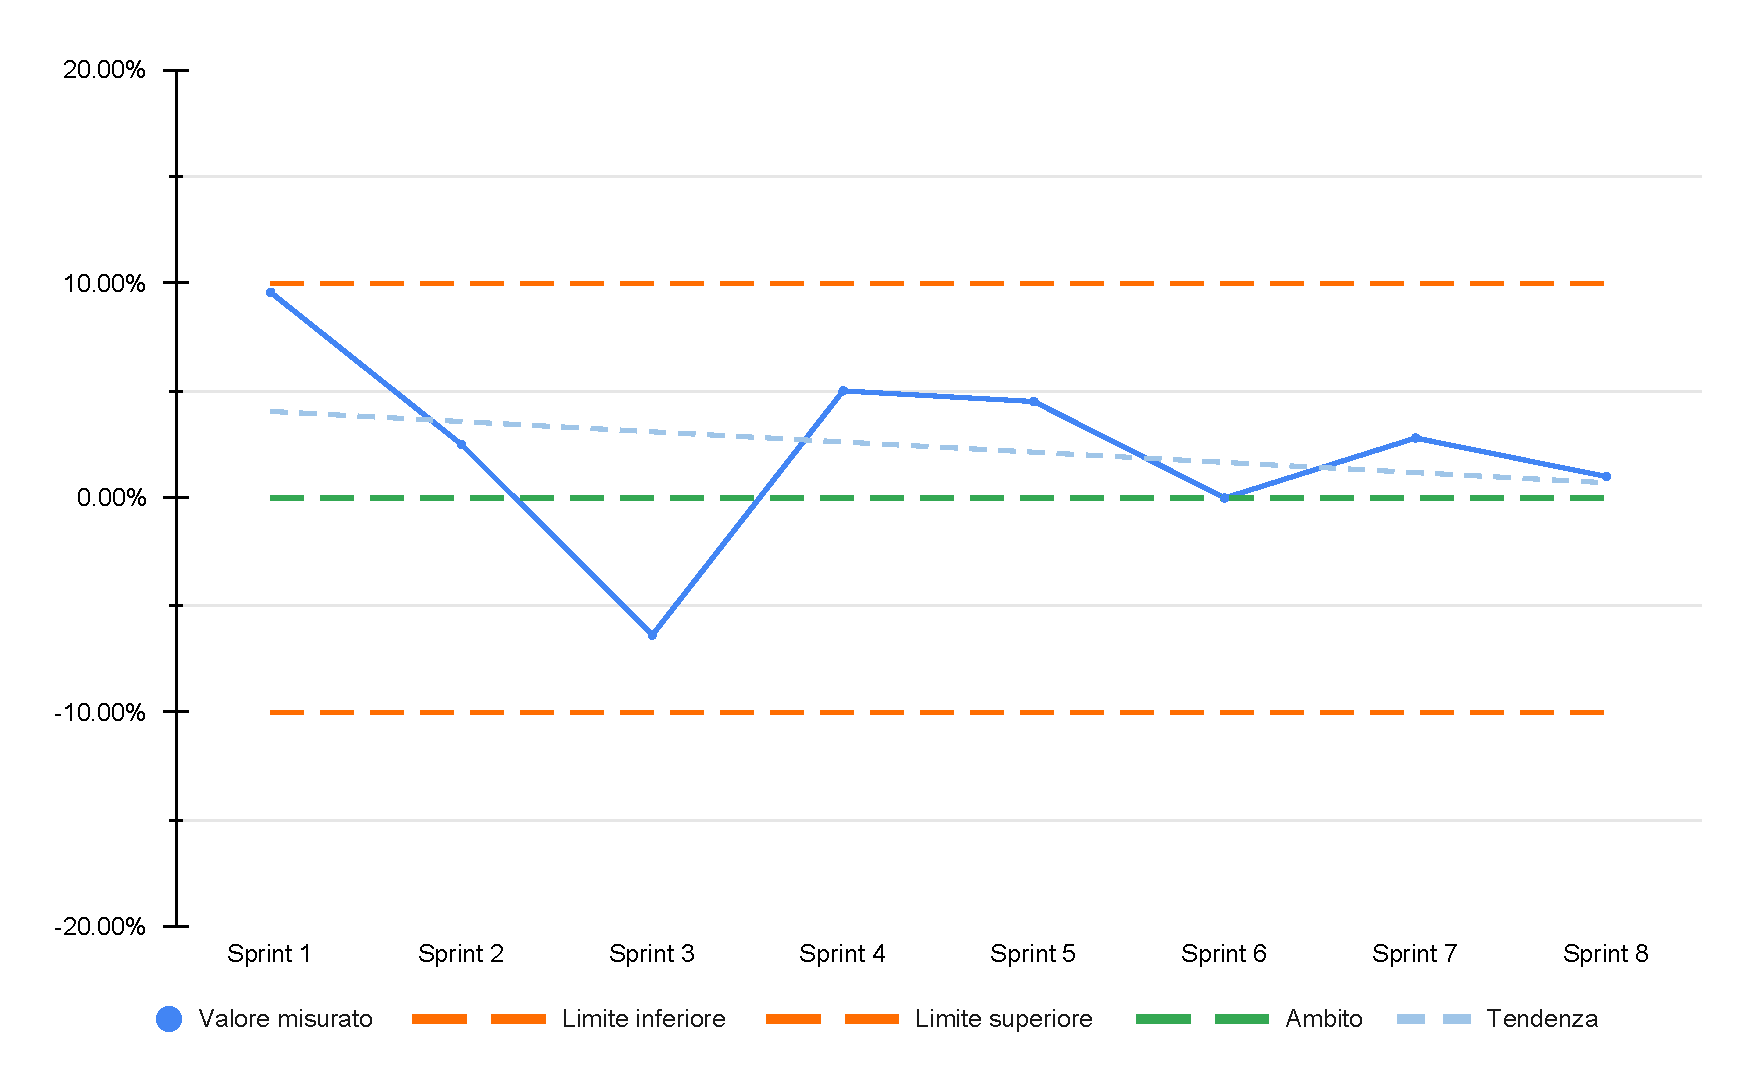
\includegraphics[width=\textwidth]{assets/variazione_budget.pdf}
    \caption{M.PC.6 - Variazione del budget tra preventivo e consuntivo}
\end{figure}

\par Nel primo \glossario{sprint}, il gruppo ha sovrastimato il carico di lavoro necessario per svolgere le attività assegnate al ruolo di analista; pertanto, i costi effettivi sono risultati inferiori rispetto a quanto preventivato. La medesima situazione si è verificata nel terzo sprint, ma con risultato opposto. La progettazione e l’implementazione delle funzionalità del \glossario{PoC} (correlate alla libreria \glossario{txtai}) hanno comportato un aumento delle ore riservate ai ruoli di programmatore e progettista. Di conseguenza, il team ha superato i costi stimati. In tutte le altre iterazioni, invece, il gruppo ha lavorato rispettando i costi allocati in fase di preventivo. A differenza di altre metriche, la variazione del budget non ha mai sforato il range di tollerabilità, raggiungendo il valore ambito in concomitanza del sesto sprint. Per questo motivo, il team ha riformulato il valore tollerabile, abbassandolo da $\pm$ 15\% a $\pm$ 10\%. Nella maggior parte degli sprint, la variazione è stata maggiore di 0; ciò significa che il gruppo ha speso il proprio budget con minor velocità di quanto pianificato. L’obiettivo del team è di diminuire lo scostamento, sia in positivo che in negativo, migliorando la pianificazione dei task, la distribuzione dei ruoli e la stima oraria delle attività.
